% ======================================================================
\section{Neural-network autoencoders}
\label{sec:autoencoders}
% ======================================================================

\subsection{From nonlinear PCA to deep autoencoders}

An autoencoder (AE) parametrizes the encoder and decoder of \eqref{eq:generic}
with neural networks, $\z=\enc_{\theta}(\q)$ and $\hat{\q}=\dec_{\vartheta}(\z)$,
and trains both jointly to minimize reconstruction error through a bottleneck
of width $r$. \textcite{kramer1991nlpca} introduced this ``autoassociative''
architecture as nonlinear PCA. \textcite{baldi1989} had shown that a
\emph{linear} autoencoder trained with a squared loss has no spurious local
minima and that its optimum spans the principal subspace. A linear AE therefore
recovers the POD subspace, though not the ordered, orthogonal modes.
\textcite{hinton2006reducing} demonstrated that deep AEs can substantially
outperform PCA on image data. In fluid dynamics, \textcite{milano2002}
reproduced the POD equivalence for near-wall turbulence and showed that
nonlinear networks improved reconstruction and prediction of the near-wall
velocity field at small additional cost, a result that anticipated much of the
later literature.

\subsection{Convolutional autoencoders and nonlinear-manifold ROMs}

Fully connected AEs scale poorly with the number of grid points. Convolutional
AEs (CAEs) exploit spatial locality, weight sharing, and hierarchical
downsampling, which makes them the dominant architecture for gridded flow data.
\textcite{lee2020cae} showed that a deep CAE defines a nonlinear trial manifold
onto which the governing equations can be projected by manifold Galerkin or
manifold LSPG, with the decoder Jacobian replacing the basis matrix. The
resulting intrusive ROMs outperformed even the optimal linear subspace on
advection-dominated problems. Non-intrusive counterparts learn the latent
dynamics as well. \textcite{gonzalez2018deep} proposed convolutional recurrent
autoencoders. The DL-ROM of \textcite{fresca2021dlrom} learns both the trial
manifold and the reduced dynamics with a CAE and a feedforward network, and
POD-DL-ROM \parencite{fresca2022poddlrom} first applies POD (randomized SVD)
and trains the AE on POD coefficients, which cuts training cost substantially
at little loss of accuracy. Nonlinear-manifold ROMs have also been made fast
enough for practical use with hyper-reduction, through shallow, sparsely
connected (masked) decoders \parencite{kim2022shallow} and reduced
over-collocation \parencite{romor2023overcollocation}.

For unsteady flows, the most common pattern couples a CAE with a recurrent
network trained afterwards on the latent sequence. \textcite{omata2019} used a
CAE to obtain low-dimensional representations of unsteady flow fields that
preserve spatial structure. \textcite{eivazi2020deep} combined an AE with an
LSTM and compared it with POD-based alternatives.
\textcite{hasegawa2020bluff} trained CNN-AE/LSTM models on flows around 80
randomly shaped bluff bodies and tested them on 20 unseen shapes, and
\textcite{nakamura2021channel} extended the approach to three-dimensional
minimal turbulent channel flow at $\mathrm{Re}_{\tau}=110$.
\textcite{maulik2021advection} showed that a two-dimensional CAE latent space
suffices to reproduce a sharp advecting shock of the viscous Burgers equation,
and a six-dimensional one the inviscid shallow-water equations. They concluded
that such advection-dominated systems are more amenable to CAE--RNN models than
to POD--Galerkin models.
\textcite{xu2020multilevel} nested a spatial CAE, a temporal convolutional AE,
and a multilayer perceptron for parametric prediction of spatio-temporal
dynamics. \textcite{racca2023caesn} paired a CAE with an echo state network to
forecast turbulent dynamics.

A parallel line of work uses AEs to interpret flows. The mode-decomposing CAE
of \textcite{murata2020mdcnn} decodes each latent variable separately and sums
the results, yielding nonlinear analogues of POD modes. For the cylinder wake
at $\mathrm{Re}_D=100$, two such modes reconstructed the flow with lower error
than two POD modes, and each nonlinear mode was found to contain several
orthogonal POD bases. The hierarchical AE of
\textcite{fukami2020hierarchical} additionally orders latent variables by their
contribution, in the spirit of POD energy ranking; it was applied to cylinder
wakes and to cross-sections of turbulent channel flow at $\mathrm{Re}_{\tau}=180$.
\textcite{page2021revealing} showed that CAE embeddings of two-dimensional
turbulence are closely associated with the simple invariant solutions of the
attractor, and introduced a latent Fourier analysis to decode physically
meaningful patterns. \textcite{fukami2023extreme} used a lift-augmented
autoencoder to compress the vortical flow of extreme gust--wing interactions,
over both time and a large gust-parameter space, to only three latent
variables. \textcite{agostini2020}
gives a tutorial-style account of AEs for exploring and predicting flow
dynamics.

\paragraph{How much does nonlinearity buy?}
\Cref{fig:ae_vs_pod} reproduces the canonical argument for nonlinear reduction on
the advected Gaussian pulse of \cref{fig:nwidth}. The data form a
one-parameter family, and a small fully connected AE with $r=2$ reconstructs
held-out snapshots with a relative error of about $3\times10^{-3}$, where POD
with the same $r$ has an error of 0.8. The learned latent trajectory
(\cref{fig:ae_vs_pod}c) is a smooth curve parametrized by the pulse position.
The same figure also shows two less advertised facts. First, the AE error
plateaus at the few-$10^{-3}$ level as $r$ increases, whereas POD converges
rapidly once $r$ exceeds the effective width of the family (here, $r\gtrsim30$).
Reaching high accuracy with a learned decoder is limited by optimization and
by the spectral bias of neural networks toward smooth functions
\parencite{rahaman2019spectral,tancik2020fourier}. Second, the AE results are the best of three
random initializations. At $r=2$ one of the three failed to find a good
embedding (error $\approx0.1$), and at $r=1$, although a single coordinate
suffices in principle, none reached an error below 0.15. POD has no such
variance. These observations are consistent with systematic comparisons
showing that the best architecture depends on the latent dimension and the
structure of the data, and that CAEs are not uniformly superior to linear or
simpler networks \parencite{gruber2022comparison}.

\begin{figure}[tbp]
  \centering
  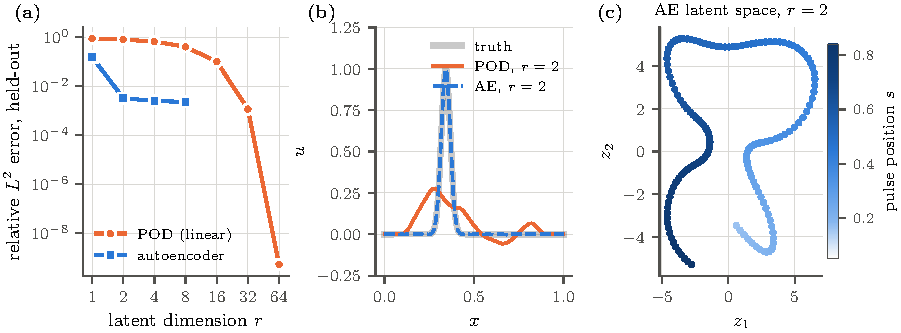
\includegraphics[width=\textwidth]{figs/ae_vs_pod.pdf}
  \caption{Linear versus nonlinear reduction of the advected Gaussian pulse
  (800 training snapshots with random positions, 150 held-out).
  (a)~Held-out relative error of POD and of a fully connected autoencoder
  ($256\!\to\!128\!\to\!64\!\to\!r$, GELU activations; best of three
  initializations) versus latent dimension. (b)~Reconstruction of a held-out
  snapshot with $r=2$. (c)~Latent coordinates of the $r=2$ autoencoder for the
  held-out set, colored by pulse position: the one-parameter family is
  embedded as a smooth curve.}
  \label{fig:ae_vs_pod}
\end{figure}

\subsection{Probabilistic, disentangled, and discrete latent spaces}

The variational autoencoder (VAE) \parencite{kingma2014vae} treats $\z$ as a
random variable with prior $p(\z)=\mathcal{N}(\bm{0},\bm{I})$ and trains an
encoder $q_{\theta}(\z\mid\q)$ and decoder $p_{\vartheta}(\q\mid\z)$ by
maximizing the evidence lower bound. The $\beta$-VAE \parencite{higgins2017betavae}
reweights the Kullback--Leibler term,
\begin{equation}
  \mathcal{L}_{\beta}=\mathbb{E}_{q_{\theta}(\z\mid\q)}\bigl[\log p_{\vartheta}(\q\mid\z)\bigr]
  -\beta\,D_{\mathrm{KL}}\bigl(q_{\theta}(\z\mid\q)\,\|\,p(\z)\bigr),
\end{equation}
and for $\beta>1$ encourages statistically independent, ``disentangled''
latent variables at some cost in reconstruction
\parencite{burgess2018understanding}. In fluids, \textcite{eivazi2022betavae}
used a convolutional $\beta$-VAE to extract a minimal, near-orthogonal set of
nonlinear modes from turbulent flow through a simplified urban environment,
together with an algorithm to rank the modes by contribution.
\textcite{solera2024betavae} combined a $\beta$-VAE with a transformer for a
two-dimensional viscous flow in periodic and chaotic regimes. The
near-orthogonal latent variables resembled POD modes but were more efficient,
and Poincar\'e maps showed that the latent dynamics captured the underlying
attractor. \textcite{wang2024optimal} examined the choice of $\beta$ and latent
dimension for such $\beta$-VAE--transformer models of turbulent flows. The
emphasis of this line of work is the \emph{quality of the latent space for
dynamics} (P3, P6), not reconstruction alone.

Discrete latent spaces are obtained with vector quantization (VQ-VAE)
\parencite{vandenoord2017vqvae}. \textcite{momenifar2022vq} used a
physics-informed VQ model, with incompressibility and velocity-gradient
statistics built into training, to compress DNS data of isotropic turbulence.
Compression for storage is itself an important application.
\textcite{glaws2020insitu} developed an AE for in situ compression of
three-dimensional turbulence. It outperformed a randomized single-pass SVD in
turbulent kinetic energy, enstrophy, and Reynolds stresses at lower cost.
\textcite{mohan2019ccl} combined convolutional compression with a convolutional
LSTM to model three-dimensional turbulence in a compressed space.

\subsection{Choosing the latent dimension}

Unlike POD, an AE provides no spectrum from which to read off a truncation.
Common practice is to scan $r$ and look for a knee in the reconstruction
error, which \textcite{linot2020inertial,linot2022node} used to estimate
inertial-manifold dimensions for the Kuramoto--Sivashinsky equation and
\textcite{linot2023couette} for minimal-flow-unit plane Couette flow at
$\mathrm{Re}=400$. Architectural regularization can make the choice
automatic. The implicit rank-minimizing AE \parencite{jing2020irmae} inserts
linear layers in the bottleneck, which bias training toward low-rank latent
codes. \textcite{zeng2024autoencoders} combined this implicit regularization
with weight decay to estimate the manifold dimension and to produce an
orthogonal manifold coordinate system. Hybrid architectures that first
subtract a PCA projection and learn only a nonlinear correction
\parencite{linot2020inertial} both reduce training cost and make the
linear--nonlinear trade-off explicit.

\subsection{Physics-constrained autoencoders}

Several approaches build physical structure into AEs. Deep Conservation
\parencite{lee2021deepconservation} constrains the latent dynamics so that
the decoded state satisfies conservation laws exactly over subdomains.
\textcite{mohan2020embedding} enforced incompressibility by construction in
convolutional networks for coarse-graining three-dimensional turbulence, using
ideas from numerical methods. Soft constraints in the loss, such as penalties
on mass and momentum conservation \parencite{lee2019cylinder} or on PDE
residuals as in physics-informed neural networks \parencite{raissi2019pinn},
are simpler but guarantee nothing. The manifold Galerkin and LSPG projections
of \textcite{lee2020cae} use the AE only for the representation and enforce the
governing equations in the dynamics, the most direct link between learned
representations and classical ROM theory.

\subsection{Practical considerations}

Deep AEs are the most expressive DR tool in this review, but their advantages
come with costs. (i)~Training is expensive and non-convex; results depend on
architecture, initialization, and optimizer, and should be reported with
variability across seeds. (ii)~Fully connected layers scale with $N$, and
convolutional layers require structured grids. Mesh-agnostic alternatives are
discussed in \cref{sec:meshfree}. (iii)~Reconstruction accuracy saturates, and
small scales are learned last \parencite{rahaman2019spectral}, which matters for
turbulence statistics and spectra. (iv)~Latent coordinates are unique only up
to diffeomorphism, and unordered unless ordering is imposed
\parencite{fukami2020hierarchical,eivazi2022betavae}. (v)~Generalization to
unseen parameters or operating conditions is often the weakest point and
should be tested explicitly (P1). Many of these issues are mitigated by POD
preprocessing \parencite{fresca2022poddlrom} or by hybrid linear--nonlinear
designs \parencite{linot2020inertial}, which suggests that linear and nonlinear
reduction are complementary rather than competing.
